\section{Model Selection}
Choosing the ML model that works the best for a given problem is a key factor for good results but it can be very time consuming. The following pages present the results obtained with several ML algorithms. Each method will be briefly introduced and tested using the training dataset. The results are analysed using three different tools:
\begin{itemize}
    \item Confusion matrix
    \item Precision, recall and F1 score
    \item ROC AUC Score
\end{itemize}
These three tools are presented and explained in Section \ref{model_tuning}.\\
Knowing the data is labeled all the methods but the last one are based on supervised learning.\\
Moreover it has already been demonstrated in Section \ref{balance_classes} that balancing classes dramatically improves results so the ML models are tested with an augmented training dataset containing duplicated individuals.

% \subsection{Stochastic Gradient Descent}

\subsection{Naive Bayes Classifier}
Naive Bayes classifiers use Bayes'theorem making the "naive" assumption that every pair of features are independant given the value of the class variable \cite{nbc_scikit} (i.e. \(P(x_i | y, x_1,..., x_{i-1}, x_{i+1},..., x_n) = P(x_i | y)\) ) leading to the following equality:
\[ P(y | x_1,..., x_n) = \frac{P(y)P(x_1,..., x_n | y)}{P(x_1,..., x_n)} = \frac{P(y)\prod_{i=1}^n P(x_i | y)}{P(x_1,..., x_n)} \]

The following results correspond to a Gaussian Naive Bayes\cite{nbcg_scikit} classifier that is very common when dealing with numerical continuous values. However it also assumes that every features follows a Gaussian distribution.\\

The confusion matrix in Figure \ref{nbd} shows poor results. This is expected because Figure \ref{data_analysis_1} demonstrates some features do not follow a Gaussian distribution. In addition, the assumption that features are independant from one another might not be relevant with this dataset. For instance, the \textit{snap\_ring\_peak\_force} might increase with the value of \textit{anlge\_1}.

\begin{figure}
    \center
    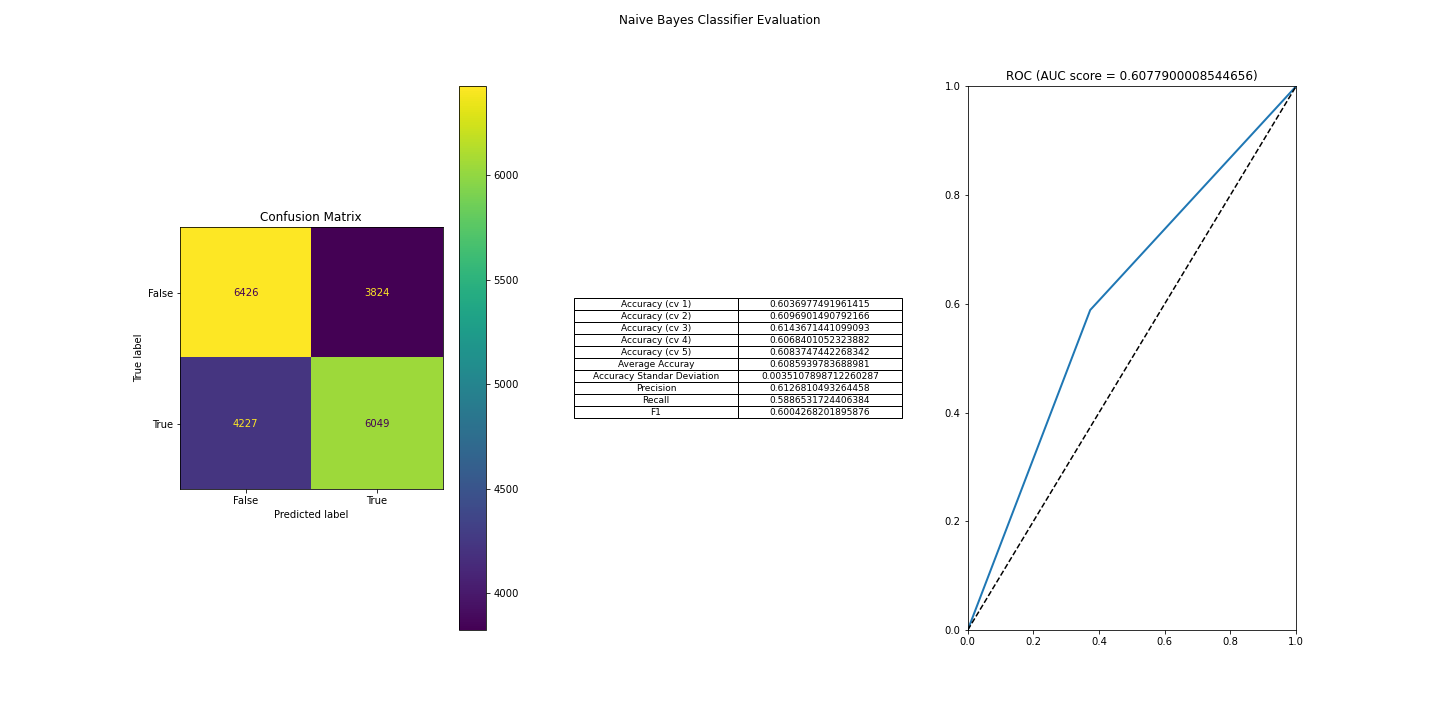
\includegraphics[scale=0.32]{img/nbc_d.png}
    \caption{Naive Bayes Classifier Evaluation}
    \label{nbc}
\end{figure}

\subsection{k-Nearest Neighbors}
The k-nearest neighbors algorithm works by classifiying an individual by looking at its neighbors\cite{knn_wikipedia}. The classifier simply look at the \(k\) nearest neighbors of the individual in the training population and attributes the class that correspond the best to the neighbors (the neighbors vote for their class, each vote is weighted either evenly accros the neighbors or according to the distance between the individual and the voting neighbor\cite{knn_scikit}).\\

When trained on the balanced dataset with removed individuals, the k-Nearest Naighbors algorithms managed to perform worse than a random classifier. But as soon as there is more individuals to learn on (with the dataset containing duplicated individuals), the algorithm performs very well (Figure \ref{knn}). Using cross-validation, the average precision is close to 0.98 and the average recall is simply 1 (with very little deviation in each case). This means the classifier is able to make really good predictions (when it finds a defective individual it is correct about 98\% of the times) while not missing any defective individual.\\
The latter might be very interesting for real world application as the company would rather manually check a item identified as defective and find out it is not defective rather than missing defective ones.

\begin{figure}
    \center
    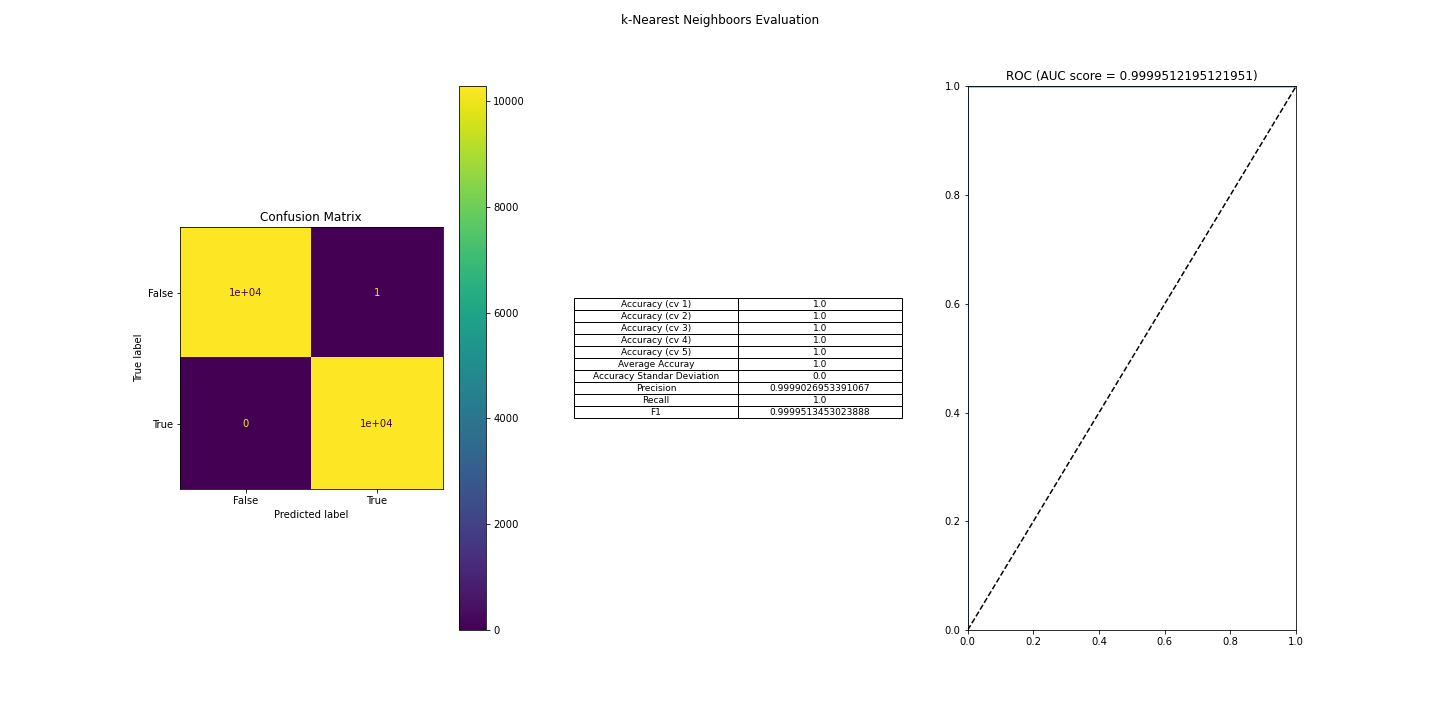
\includegraphics[scale=0.32]{img/knn_d.png}
    \caption{k-Nearest Neighbors Evaluation}
    \label{knn}
\end{figure}

\subsection{Random Forest Classifier}
Random Forest Classifier works by creating multiple Decision Trees on various subsets of the data, the decision of the forest for classification is simply the class that has been predicted by most of the trees\cite{rdf_wikipedia}. A Decision Tree is built by finding the rule which devide the best the population of each node, this can be the rule that isolate most individuals from the same class (this method is called information gain and is based on the concept of entropy)\cite{dtl_wikipedia}. A node cannot be devided when there are not enough individuals (in the node or in the to-be-created child-node), then the leaf is labeled with the class with the most representants on the node.\\

Random Forest Classifiers have a \textit{class\_weight} attribute in Scikit-Learn in order to address imbalance between classes\cite{rfc_scikit}. However it seemed to perform worse than training the forest with the dataset containing duplicates (Figure \ref{rfc_w}). Figure \ref{rfc} shows stunning results: sturdy precision and recall of 1 accross all cross validations.\\

While these results look great for now it remains to be seen if the forest is actually able to adapt to other errors. It is very likely that the classifier is now over-fitting both classes. By duplicating individuals, the model might learn that only these items are defective and will not be able to detect slightly different defective items.\\

\begin{figure}
    \center
    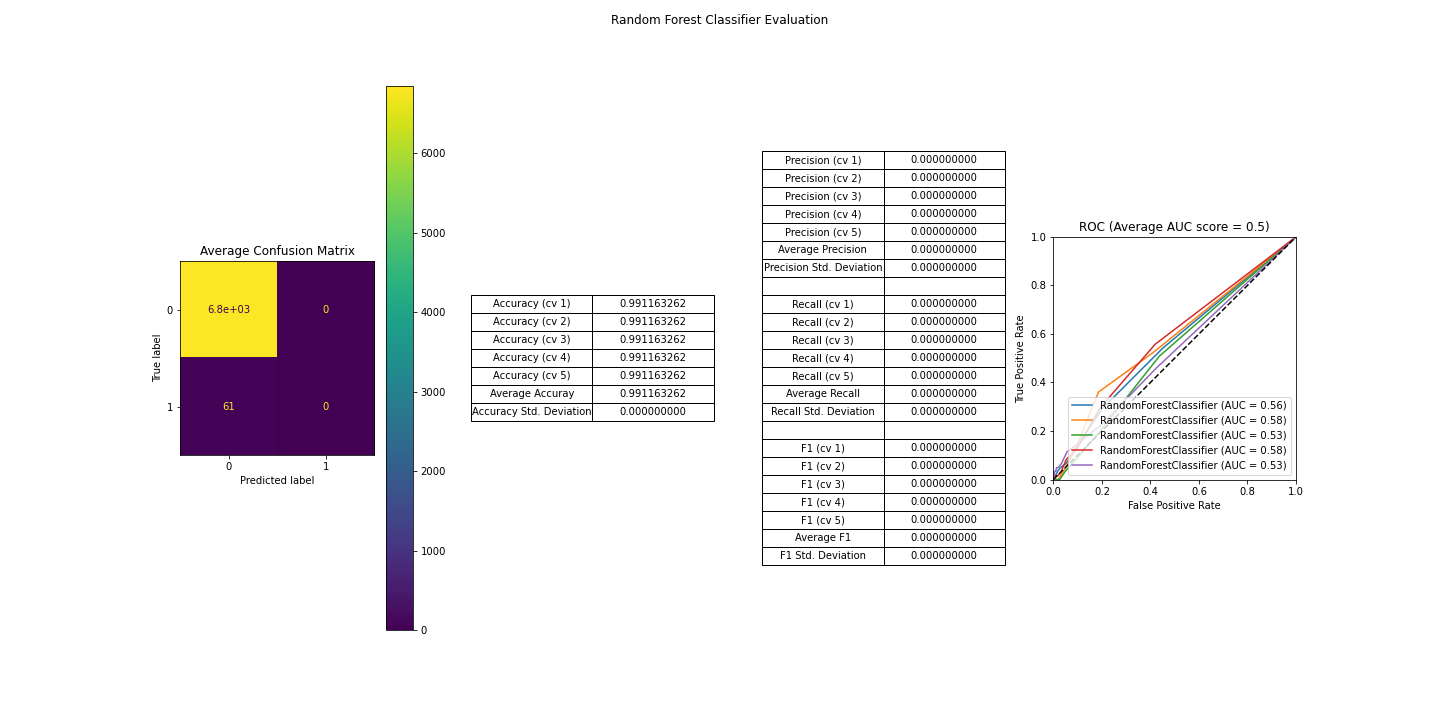
\includegraphics[scale=0.32]{img/rfc_w.png}
    \caption{Random Forest Classifier Evaluation (with \textit{class\_weight} set to \textit{"balanced"} )}
    \label{rfc_w}
\end{figure}

\begin{figure}
    \center
    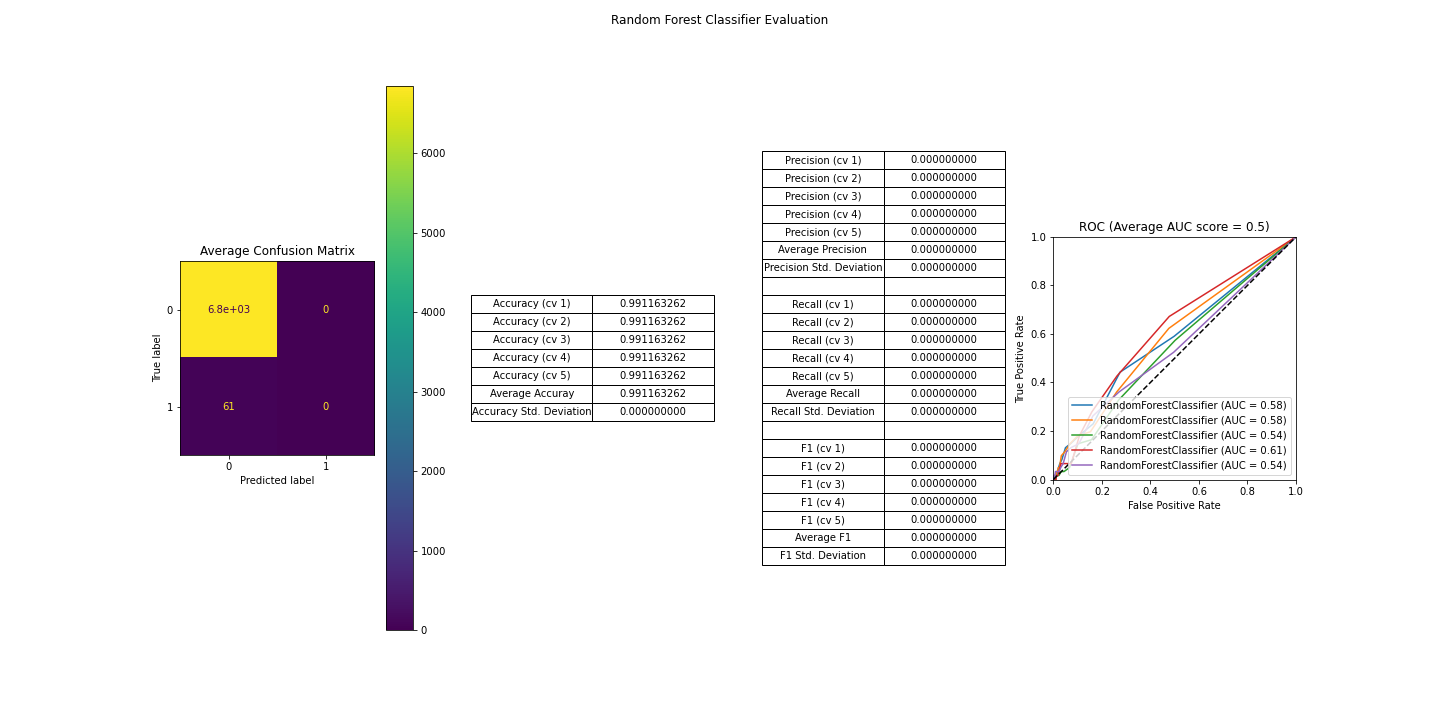
\includegraphics[scale=0.32]{img/rfc_d.png}
    \caption{Random Forest Classifier Evaluation}
    \label{rfc}
\end{figure}

\subsection{Multi-Layer Perceptron}

\subsection{Novelty Detection}